\chapter{Testing and Validation}
\label{chap:testing}

\section{Testing Strategy}
FORGE mixes a game engine, procedural generation and machine learning, so testing runs at four levels:
\begin{enumerate}
    \item \textbf{Unit tests:} maths and data handling (observation and action mapping, archetype mix, $CR_0$, telemetry schema, Judge target and features) in \texttt{pytest} and headless GDScript.
    \item \textbf{Engine integration tests:} headless GDScript tests that load the real game scene (damage telemetry, cold start, archetypes, swarm rooms, overlay sync, playtest flow, SQLite).
    \item \textbf{Solvability tests:} 500 seeds for each room count from 3 to 9 (3,500 layouts) in headless Godot in CI.
    \item \textbf{Model evaluation:} the PPO policy against baselines in simulation, and the Judge against the linear formula on held-out simulated players and on the real pilot floors.
\end{enumerate}

\section{Test Levels and Techniques}
\begin{table}[!htbp]
\centering
\caption{FORGE test levels}
\label{tab:test_levels}
\small
\begin{tabular}{p{0.20\textwidth}p{0.26\textwidth}p{0.26\textwidth}p{0.20\textwidth}}
\toprule
\textbf{Level} & \textbf{Scope} & \textbf{Tool} & \textbf{Where} \\
\midrule
Unit & Maths, schema, Judge & \texttt{pytest} (137 test functions in 11 files), headless GDScript & Local and CI \\
Integration & Real game scene & 11 headless GDScript tests + SQLite test & CI (Godot 4.7.2) \\
Solvability & Layout reachability and structure & \texttt{ci\_solvability\_runner.gd} & CI \\
Model evaluation & PPO and Judge & \texttt{evaluate\_policies.py}, \texttt{train\_judge.py} & Python 3.12 \\
Manual & Feel, visuals, playtest & Supervised play, playtest build & Dev PC \\
\bottomrule
\end{tabular}
\end{table}

The solvability harness now checks more than reachability: the requested room count, no overlapping rooms or corridors, the exit at maximum depth (and depth at least 2), room sizes within bounds, and at least 6 distinct sizes per 100 rooms.

\section{Test Cases}
Table~\ref{tab:test_cases} lists the main test cases. TC-01 to TC-10 come from Mid-1; TC-11 to TC-17 are new. Appendix~\ref{app:test_cases} maps them to the test files.

\begin{table}[!htbp]
\centering
\caption{Main test cases and results}
\label{tab:test_cases}
\scriptsize
\begin{tabular}{p{0.06\textwidth}p{0.16\textwidth}p{0.42\textwidth}p{0.10\textwidth}p{0.12\textwidth}}
\toprule
\textbf{ID} & \textbf{Component} & \textbf{What is checked} & \textbf{Type} & \textbf{Result} \\
\midrule
TC-01 & TelemetryLogger & Damage taken/dealt recorded exactly in the real scene & Auto & Pass \\
TC-02 & Cold start & $CR_0$ and $s_0$ for three scripted profiles & Auto & Pass \\
TC-03 & PPOPolicy & 8 inputs give 8 outputs in $[-1,1]$; parity with SB3 \texttt{predict()} & Auto & Pass \\
TC-04 & PPOPolicy & Missing or wrong-shape weights trigger the heuristic, no crash & Auto/manual & Pass \\
TC-05 & DifficultyManager & Action $-1$/$+1$ maps to the exact range ends & Auto & Pass \\
TC-06 & DungeonGenerator & 3,500 layouts: reachable, no overlaps, exit depth, sizes & Auto & Pass \\
TC-07, 08 & Enemy & Crawler chase; Pyromancer telegraph and fireball & Manual & Pass \\
TC-09 & Player & No damage during dodge roll & Manual & Pass \\
TC-10 & Static baseline & $+8\%$ per floor exactly & Auto & Pass \\
TC-11 & SQLite backend & Rows written and read back with the real extension & Auto & Pass \\
TC-12 & JSON fallback & Telemetry still saved when the plugin is missing & Auto & Pass \\
TC-13 & Archetypes & Multipliers per type; mix follows $c$; Swarmer slot = 3 bodies & Auto & Pass \\
TC-14 & Playtest flow & Rating only after consent; stored per floor & Auto & Pass \\
TC-15 & Judge & Deterministic corpus; no player in both train and test; beats mean predictor; SHAP sums to prediction & Auto & Pass \\
TC-16 & Defense Overlay & Moving one slider does not re-apply the others (DEF-10) & Auto & Pass \\
TC-17 & BSP generator & 200 seeds $\times$ 4--10 rooms connected, exit reachable, no overlaps & Auto & Planned \\
\bottomrule
\end{tabular}
\end{table}

\section{Test Results}
\tofill{paste the result of the latest CI run: number of pytest tests passed, all GDScript tests PASS, 3,500/3,500 layouts}. On the last recorded run all automated tests passed. Two measurements must be refreshed for the shipped 8-output policy before the evaluation:
\begin{itemize}
    \item \textbf{Inference latency (NFR-06):} at Mid-1 the 7-output policy took a mean of $0.21$\,ms on the development PC. The benchmark (\texttt{tests/benchmark\_inference.gd}) is not in CI. \tofill{run it once on the dev PC with the shipped policy and report median, p95 and max; use this one number everywhere}.
    \item \textbf{Frame rate (NFR-05):} frame times are now logged per floor. \tofill{p95 and max frame time over the 29 real floors, and the machine used}.
\end{itemize}

\section{Simulated Policy Evaluation (simulator v3)}
\label{sec:sim_results}\label{sec:policy_eval}
\textbf{Protocol.} Six simulated player profiles (starting skill 0.10, 0.20, 0.45, 0.70, 0.80, 0.90). For each, 100 paired episodes of 30 floors; every policy meets the same player and the same random noise. Compared: the shipped policy, a random untrained policy (average of 10), the rule-based heuristic and the static $+8\%$ baseline. Pacing error is $|t_{room} - 7.5\,\text{s}| / 7.5\,\text{s}$ (the DER of SC-07).

\begin{table}[!htbp]
\centering
\caption{Shipped policy vs.\ baselines in simulator v3 (100 paired episodes per profile)}
\label{tab:policy_eval}
\scriptsize
\begin{tabular}{lcccccccc}
\toprule
& \multicolumn{4}{c}{\textbf{Reward per floor (higher is better)}} & \multicolumn{4}{c}{\textbf{Pacing error (lower is better)}} \\
\cmidrule(lr){2-5}\cmidrule(lr){6-9}
\textbf{Profile (skill)} & PPO & Random & Heuristic & Static & PPO & Random & Heuristic & Static \\
\midrule
Novice (0.10) & \textbf{0.473} & $-1.434$ & $-0.158$ & $-3.258$ & \textbf{0.130} & 0.871 & 0.378 & 1.499 \\
Novice (0.20) & \textbf{0.522} & $-0.917$ & $-0.029$ & $-2.651$ & \textbf{0.134} & 0.658 & 0.327 & 1.287 \\
Mid (0.45) & \textbf{0.562} & 0.187 & 0.231 & $-1.177$ & \textbf{0.132} & 0.259 & 0.206 & 0.722 \\
Skilled (0.70) & \textbf{0.550} & 0.093 & 0.152 & $-0.391$ & \textbf{0.122} & 0.204 & 0.148 & 0.348 \\
Expert (0.80) & \textbf{0.546} & $-0.115$ & 0.074 & $-0.371$ & \textbf{0.124} & 0.257 & 0.150 & 0.297 \\
Expert (0.90) & \textbf{0.531} & $-0.309$ & $-0.031$ & $-0.452$ & \textbf{0.125} & 0.305 & 0.171 & 0.284 \\
\bottomrule
\end{tabular}
\end{table}

\textbf{Results.} The shipped policy is better than all three baselines on both reward and pacing error for all six profiles (paired tests, all $p < 10^{-11}$). Its pacing error is $0.12$--$0.13$, inside the $0.15$ target for every profile, with 0 deaths per floor. The static baseline kills novices about 0.7 times per floor.

\textbf{Every output is now used.} Unlike Mid-1, the policy now changes every setting with skill. From skill 0.10 to 0.90, mean enemy health goes from 22.7 to 79.9, damage from 20.6 to 31.0, hazard density from 0.36 to 0.74, scarcity from 0.31 to 0.69, rooms from 6.1 to 8.5, and archetype complexity $c$ from 0.32 to 0.79 (novices get mostly Swarmers and Pyromancers, experts mostly Brutes and Skirmishers). No output sits within 5\% of a range end for all profiles, and the learned action spread is below 0.25 for every output.

\begin{figure}[!htbp]
\centering
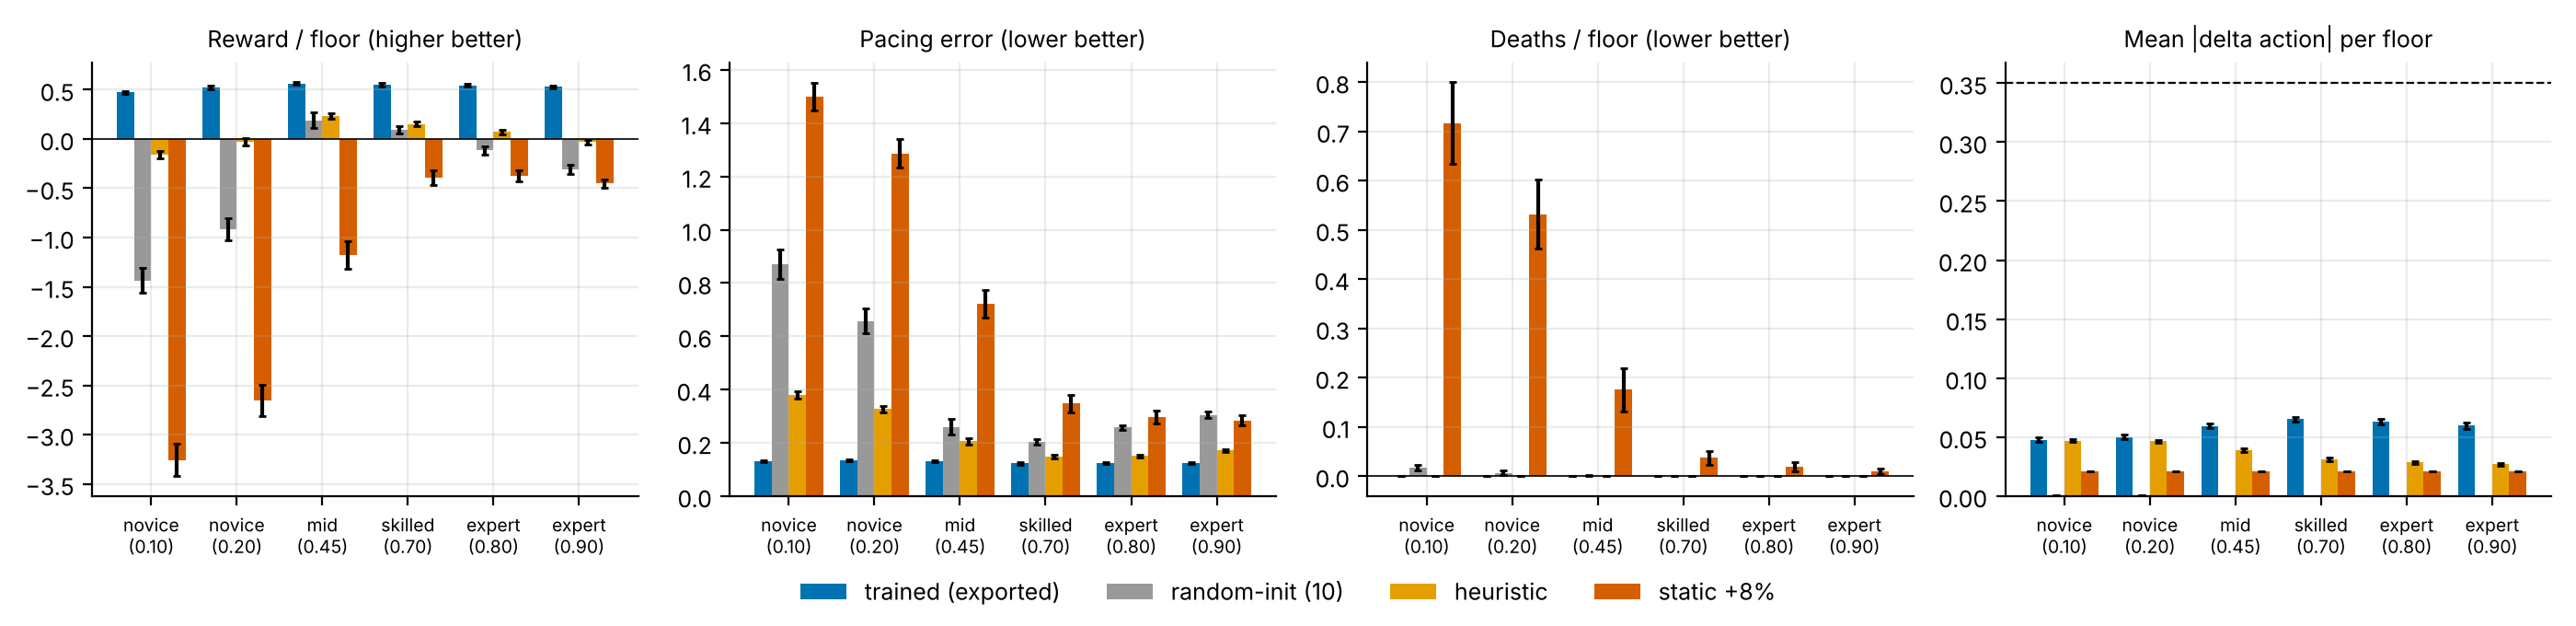
\includegraphics[width=\textwidth]{ThesisFigs/fig_policy_eval_v3.png}
\caption{Reward and pacing error per simulated profile, simulator v3}
\label{fig:policy_eval}
\end{figure}

\subsection{Convergence and Stability (abrupt skill change)}
\label{sec:shift_test}
To test the committee's question about abrupt changes, the player's skill drops by 0.30 at floor 10 and comes back at floor 20. The shipped policy brings the pacing error back under 0.15 within \textbf{2 floors} after the drop (and 4 floors after the recovery) for all three tested skill paths; the heuristic and the static baseline do not recover within 10 floors on most paths. The mean change of the action per floor is $0.058$ (worst profile $0.065$), far below the $0.35$ limit, so the policy does not thrash. This suggests a separate rate limiter is not needed; we will confirm with human play.

\subsection{What these results do and do not show}
\begin{itemize}
    \item They are \textbf{simulation only}. No human comparison exists yet.
    \item Part of the personalisation comes from the reward design: several reward terms use the hidden skill, reflex and tactics (Section~\ref{sec:reward}). So the perfect rank correlation between skill and chosen difficulty (Spearman $\rho = 1.0$) is partly built in.
    \item The static $+8\%$ baseline is weak: it was never tuned and it kills novices. Beating it says little. Stronger baselines are planned: the BSP generator and a ``best fixed setting'' tuned on the whole simulated population.
    \item The adaptive condition plays five calibration floors that the static condition does not. Comparisons should report floors 6+ separately or give every condition the same first five floors.
\end{itemize}

\section{Judge Evaluation}
\label{sec:judge_results}
\textbf{Protocol.} 30,199 synthetic floors from 3,000 simulated players, split by player: 2,400 for training (5-fold grouped cross-validation) and 600 held out. Then the 29 real consented floors (3 sessions, one player) as a pilot check.

\begin{table}[!htbp]
\centering
\caption{Judge vs.\ the hand-weighted formula on 600 held-out synthetic players}
\label{tab:judge_synth}
\small
\begin{tabular}{lccc}
\toprule
\textbf{Model} & \textbf{Test MAE} & \textbf{Test RMSE} & \textbf{Test $R^2$} \\
\midrule
\textbf{LightGBM Judge (18 features)} & \textbf{0.052} & 0.076 & 0.823 \\
Linear regression, same features & 0.069 & 0.094 & 0.734 \\
Old formula, rescaled to $[0,1]$ & 0.104 & 0.135 & 0.445 \\
Old formula as is (score/100) & 0.206 & 0.242 & $-0.780$ \\
Mean predictor & 0.146 & 0.182 & 0.000 \\
\bottomrule
\end{tabular}
\end{table}

\textbf{Synthetic result:} the target (MAE $\le 0.15$ and better than the formula) is met. The Judge's error is half that of the rescaled formula, and it also beats a linear model on the same features, so it captures non-linear effects and player context.

\begin{table}[!htbp]
\centering
\caption{Pilot check on real floors (n = 29, one player; too small to conclude)}
\label{tab:judge_real}
\small
\begin{tabular}{lccc}
\toprule
\textbf{Compared against} & \textbf{Judge MAE} & \textbf{Old formula MAE} & \textbf{Mean predictor MAE} \\
\midrule
Measured difficulty (training target) & 0.121 & \textbf{0.109} & 0.148 \\
Player's own rating $(r-1)/4$ & 0.311 & \textbf{0.162} & 0.271 \\
\bottomrule
\end{tabular}
\end{table}

\textbf{Real-data result:} on these 29 floors the Judge does \emph{not} beat the old formula. It under-predicts (mean prediction 0.19 against a measured 0.29): this player took more damage on easy adaptive floors than simulator v3 expects, which is a sim-to-real gap in the simulator's damage model. The player rated almost every adaptive floor 3 of 5, while the measured target averages 0.29, so the outcome-based target is only a weak stand-in for felt difficulty (rank correlation 0.52). This is the main reason to retrain on real ratings once more players have played, and to build the player model.

\begin{figure}[!htbp]
\centering
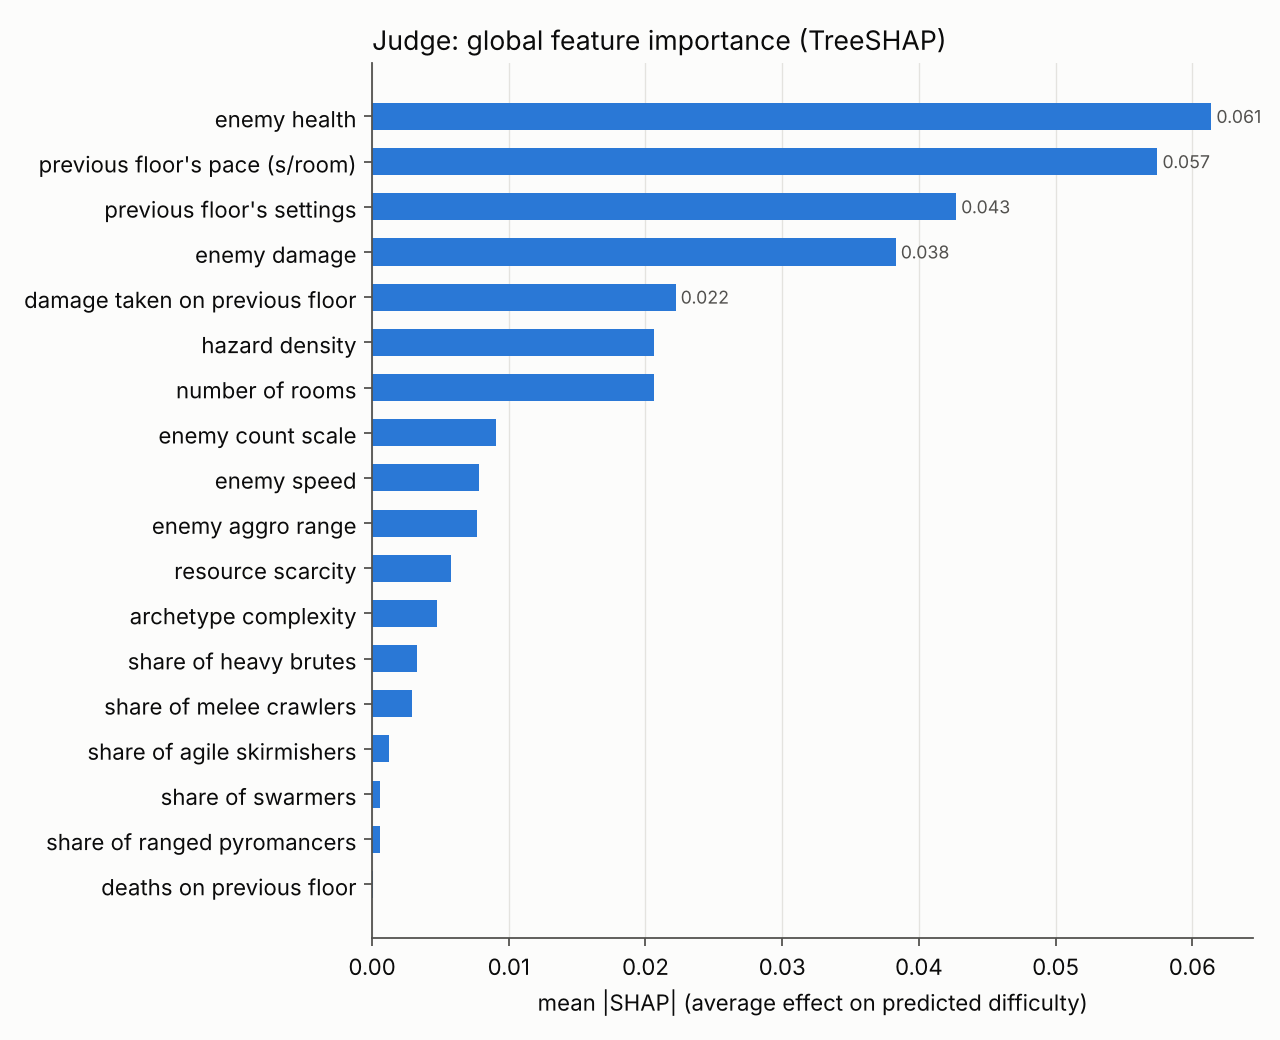
\includegraphics[width=0.75\textwidth]{ThesisFigs/judge_shap_bar.png}
\caption{Judge SHAP: mean absolute contribution per feature on 2,000 held-out synthetic floors}
\label{fig:judge_shap}
\end{figure}

\textbf{What drives difficulty (Judge SHAP).} The top features are enemy health (0.061), the previous floor's pace (0.057), the previous floor's settings (0.043), enemy damage (0.038) and damage taken on the previous floor (0.022). Player context ranks 2nd, 3rd and 5th, so the Judge predicts difficulty \emph{for this player}, not only for the settings. Because the Judge learned from the simulator, these rankings describe the simulator's view of difficulty until it is retrained on real data.

\section{Baseline Comparison Status}
Table~\ref{tab:baseline_plan} shows the comparison planned for the Final-1 evaluation. Cells marked \tofill{} are not measured yet and must not be read as results.

\begin{table}[!htbp]
\centering
\caption{Final-1 comparison table (to be completed by the evaluation script)}
\label{tab:baseline_plan}
\scriptsize
\begin{tabular}{p{0.26\textwidth}p{0.18\textwidth}p{0.18\textwidth}p{0.18\textwidth}}
\toprule
\textbf{Metric} & \textbf{FORGE (PPO)} & \textbf{Static $+8\%$} & \textbf{BSP (fixed Intermediate)} \\
\midrule
Solvability (\% of layouts) & 100\% (3,500) & 100\% (same generator) & \tofill{} \\
Pacing error, simulated (mean of 6 profiles) & 0.128 & 0.740 & \tofill{} \\
Layout diversity (pairwise layout distance) & \tofill{} & \tofill{} & \tofill{} \\
Start-to-exit path length / dead ends & \tofill{} & \tofill{} & \tofill{} \\
Floors to recover after skill drop & 2 & never (10+) & \tofill{} \\
PPO on calibrated simulator (ablation) & \tofill{} & -- & -- \\
\bottomrule
\end{tabular}
\end{table}

\section{Acceptance Testing}
The Final-1 acceptance status is in Table~\ref{tab:acceptance_criteria} and Table~\ref{tab:success_criteria}. All implemented requirements pass their tests. Open items are the BSP generator (FR-14), the ML pipeline (FR-15, FR-16) and the refreshed latency and frame-rate numbers.

\section{Edge and Failure Cases}
\begin{enumerate}
    \item \textbf{Missing or wrong policy file:} the game falls back to the 8-output heuristic. A file whose input width is not 8 is now rejected by a shape check (this was a known gap at Mid-1). An old 7-output file is accepted, and $a_7$ is derived from the difficulty score.
    \item \textbf{SQLite plugin missing:} telemetry falls back to JSON (TC-12).
    \item \textbf{Player declines consent:} no rating is asked; floors are logged with \texttt{consent = 0} and left out of analysis (TC-14).
    \item \textbf{Abrupt skill drop:} the policy recovers in 2 floors in simulation (Section~\ref{sec:shift_test}).
    \item \textbf{Overlay changes during play:} floors changed by the Defense Overlay are flagged \texttt{manual\_override} and left out of the Judge corpus.
\end{enumerate}

\section{Defects and Corrective Actions}
\label{sec:defects}
DEF-01 to DEF-09 were fixed before Mid-1 (see the Mid-1 report). New in Iteration 3:

\begin{table}[!htbp]
\centering
\caption{Defects found in Iteration 3}
\label{tab:defects}
\scriptsize
\begin{tabular}{p{0.10\textwidth}p{0.38\textwidth}p{0.44\textwidth}}
\toprule
\textbf{ID} & \textbf{Symptom} & \textbf{Fix} \\
\midrule
DEF-10 & In the Defense Overlay, updating the sliders from code re-emitted their signals, so it looked as if only enemy HP adapted. & \texttt{sync\_ui\_with\_manager()} uses \texttt{set\_value\_no\_signal}; guarded by \texttt{test\_overlay\_sync} (TC-16). \\
DEF-11 & \texttt{release.yml} still pins Godot 4.3 while CI and the project use 4.7.2. & \tofill{update release.yml to 4.7.2 and note the commit} \\
DEF-12 & The sensitivity script \texttt{ai/jh.py} applies a final $\tanh$ (the game clips) and names only 7 outputs. & \tofill{update to clip and 8 outputs before the post-retrain audit} \\
\tofill{} & \tofill{any other defects found during Iteration 3} & \\
\bottomrule
\end{tabular}
\end{table}

\section{Current Validation Status}
Validated: all implemented features have automated tests that pass; the policy beats three baselines in simulation; the Judge beats the old formula on simulated players. Not yet validated: anything with humans beyond one pilot player, the BSP comparison, and the new ML pipeline. Threats to validity are summarised in Section~\ref{sec:limitations}.
